\documentclass[letterpaper]{article}
\usepackage{underscore}
\usepackage[left=2.0cm, right=2.0cm, top=2.0cm]{geometry}
\usepackage[utf8]{inputenc}
\usepackage{graphicx}
\usepackage{graphics}
\usepackage[spanish]{babel}
\usepackage{lipsum}
\usepackage{float}
\usepackage{subfigure}
\usepackage{biblatex}
\usepackage{csquotes}
\usepackage{color}

\title{2\_5\_arreglos\_de\_amplificadores\_de\_potencia}
\author{Alcantar Diaz Joel Alejandro\\Ledesma Hernández Miguel Ángel}
\date{24/10/2019}

\begin{document}

\maketitle
\begin{center}
\begin{large}
\vspace{2cm}
    \begin{center}
        
\includegraphics[scale=0.5]{IMG/UPZMGlog.png}
    \end{center}
\vspace{2cm}
Universidad politécnica de la zona metropolitana de Guadalajara\\
Sistemas electrónicos de interfaz\\
4-A Mecatrónica\\
\end{large}
\end{center}

\newpage
\begin{large}
    \textbf{Objetivo.}\\\\
    Realizar las simulaciones de los arreglos de los Amplificadores Operacionales.\\\\
\end{large}
\begin{large}
    \textbf{Materiales.}\\\\
    Computadora con OrCad\\\\
\end{large}
\begin{large}
    \textbf{Procedimiento.}
    Para la realizacion de los circuitos en esta practica se siguieron los diagramas sugeridos por el maestro y que se presentan a continuacion.

\end{large}

%circuito 1 onda 1  cir4 ond7 

\begin{figure}[htbp]
    \centering
    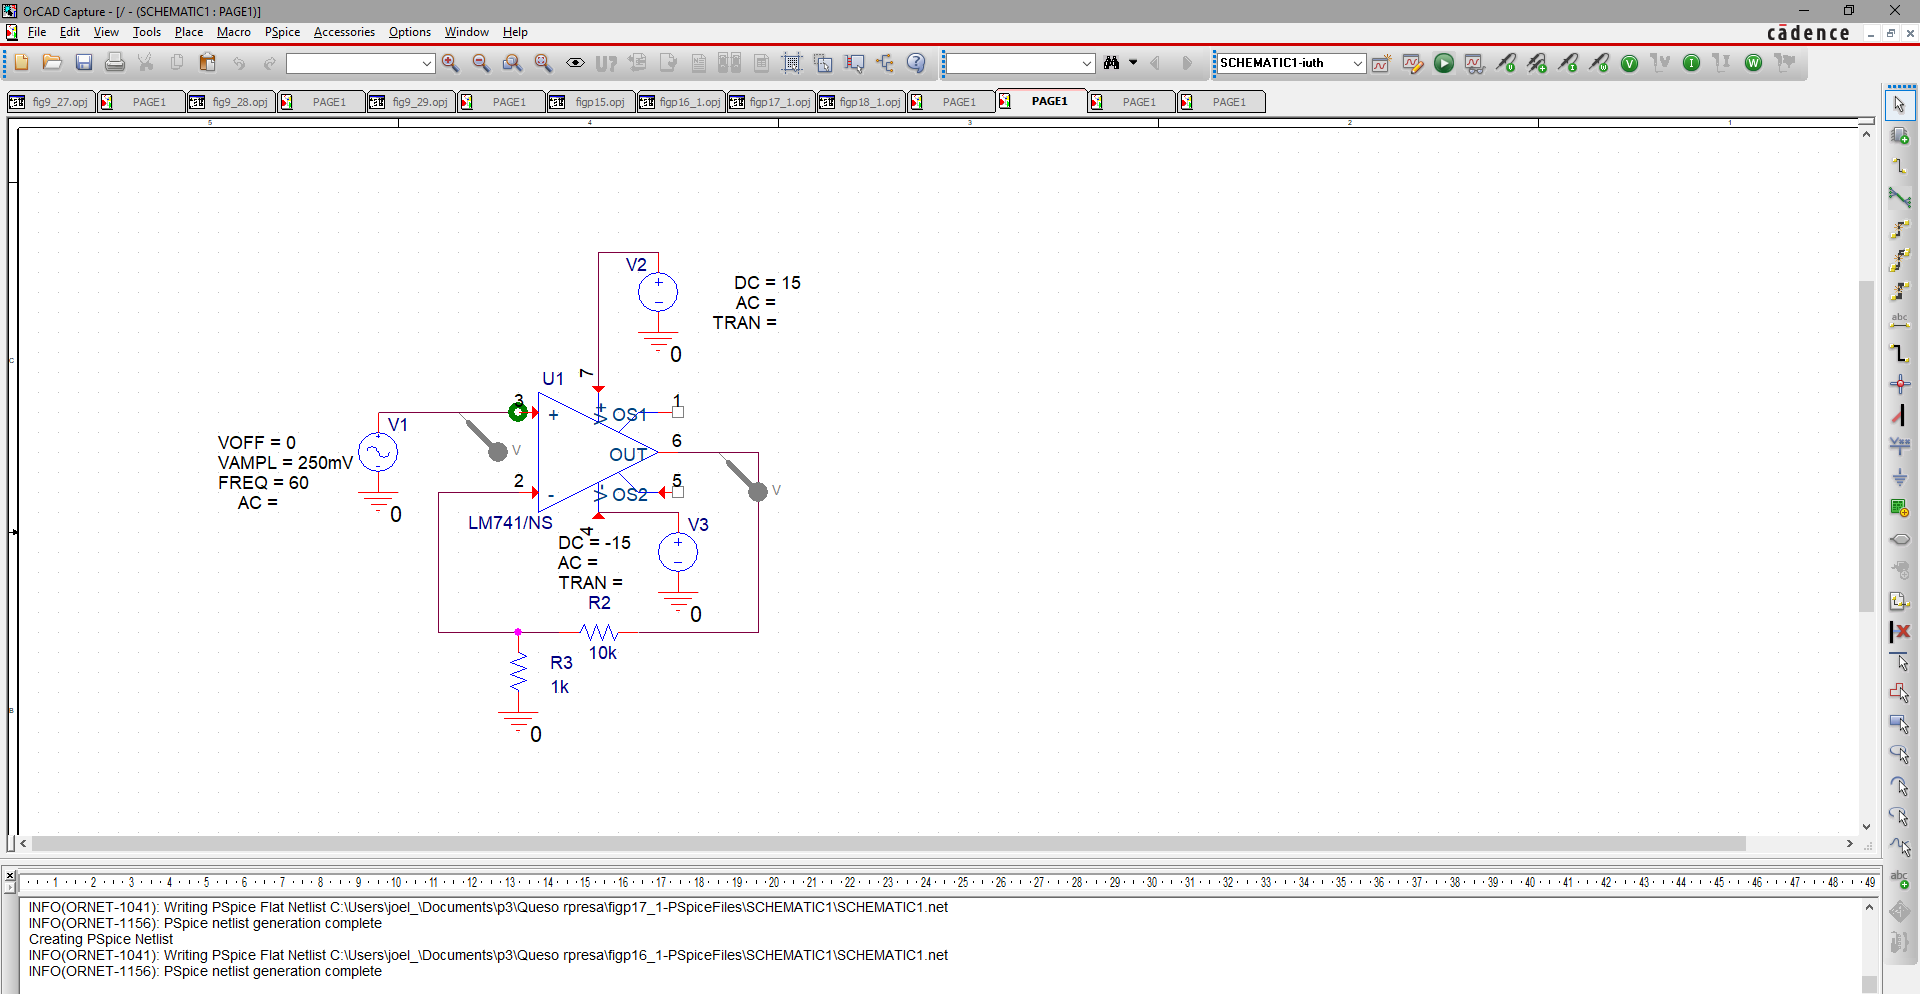
\includegraphics[width=18cm]{IMG/cir(4).png}
    \caption{Circuito 1:Inversor}
    \label{fig:my_label}
\end{figure}
\begin{figure}[htbp]
    \centering
    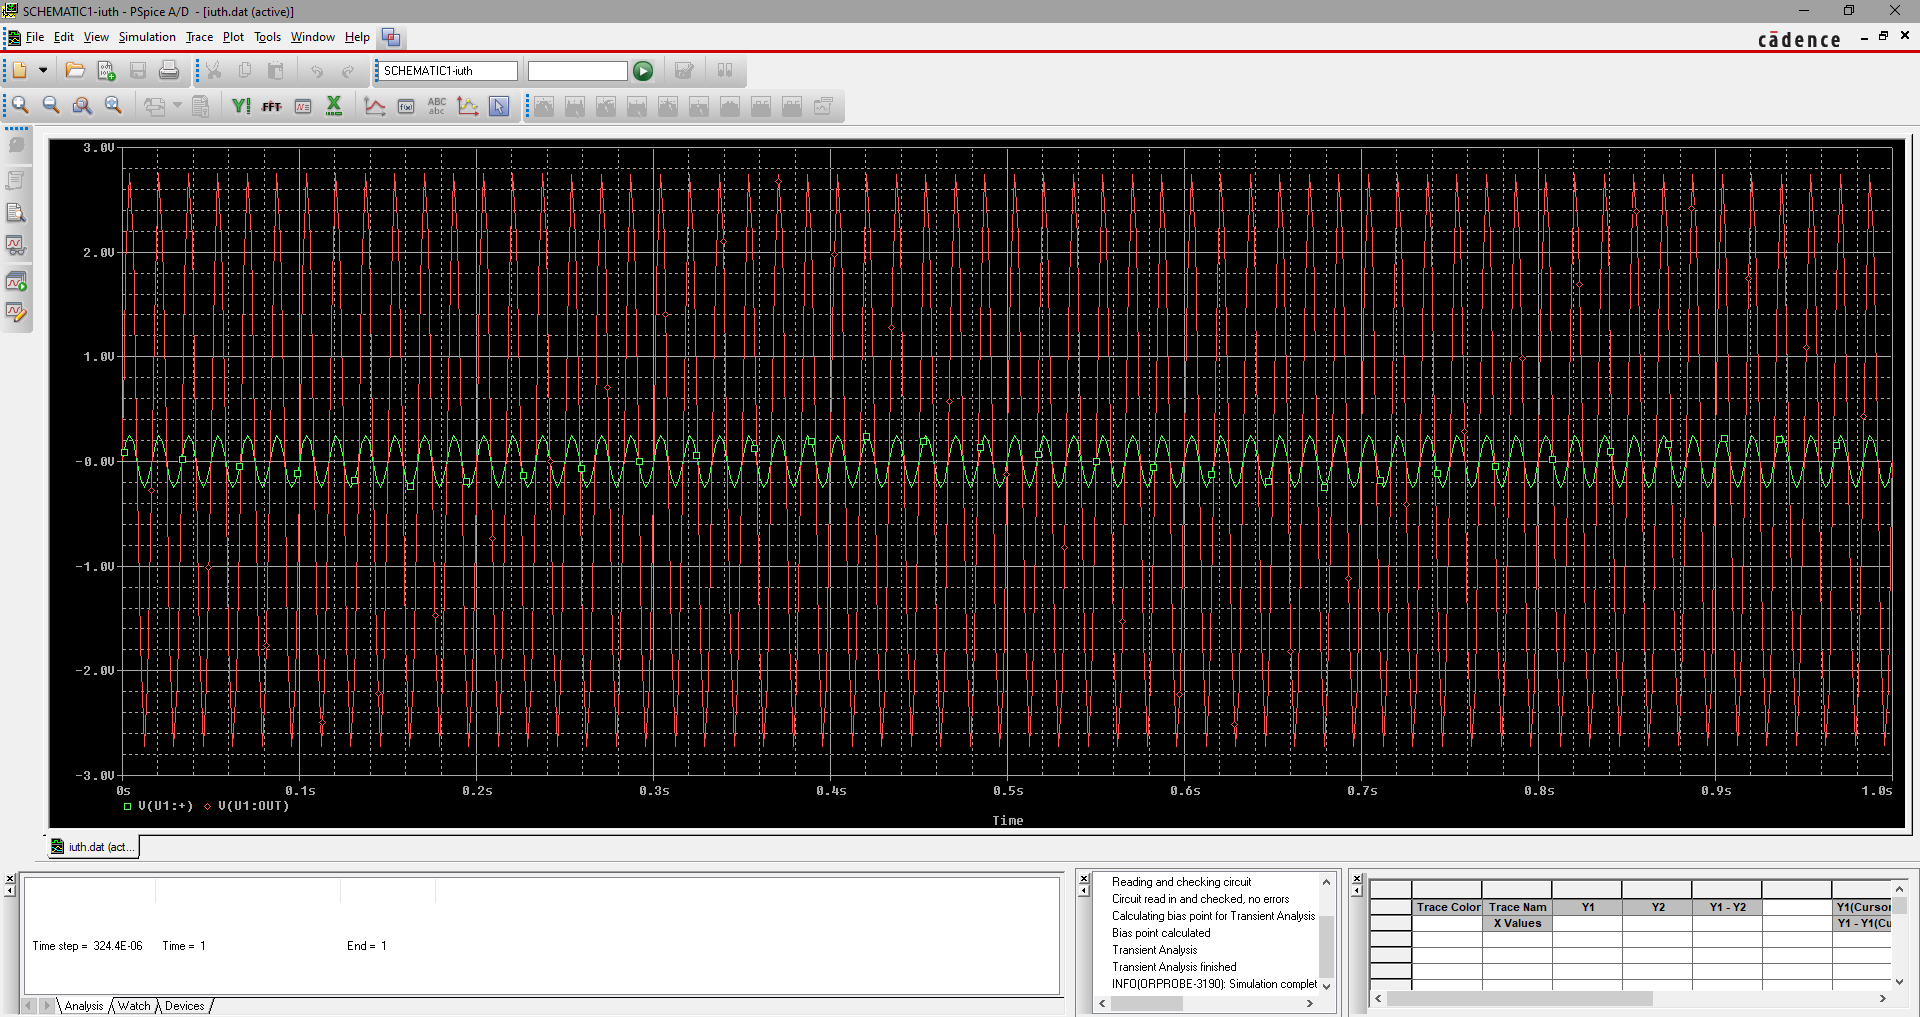
\includegraphics[width=18cm]{IMG/ond(7).png}
    \caption{Onda 1: Inversa}
    \label{fig:my_label}
\end{figure}

%circuito 2 onda 2 cir 5 ond 1
\begin{figure}[htbp]
    \centering
    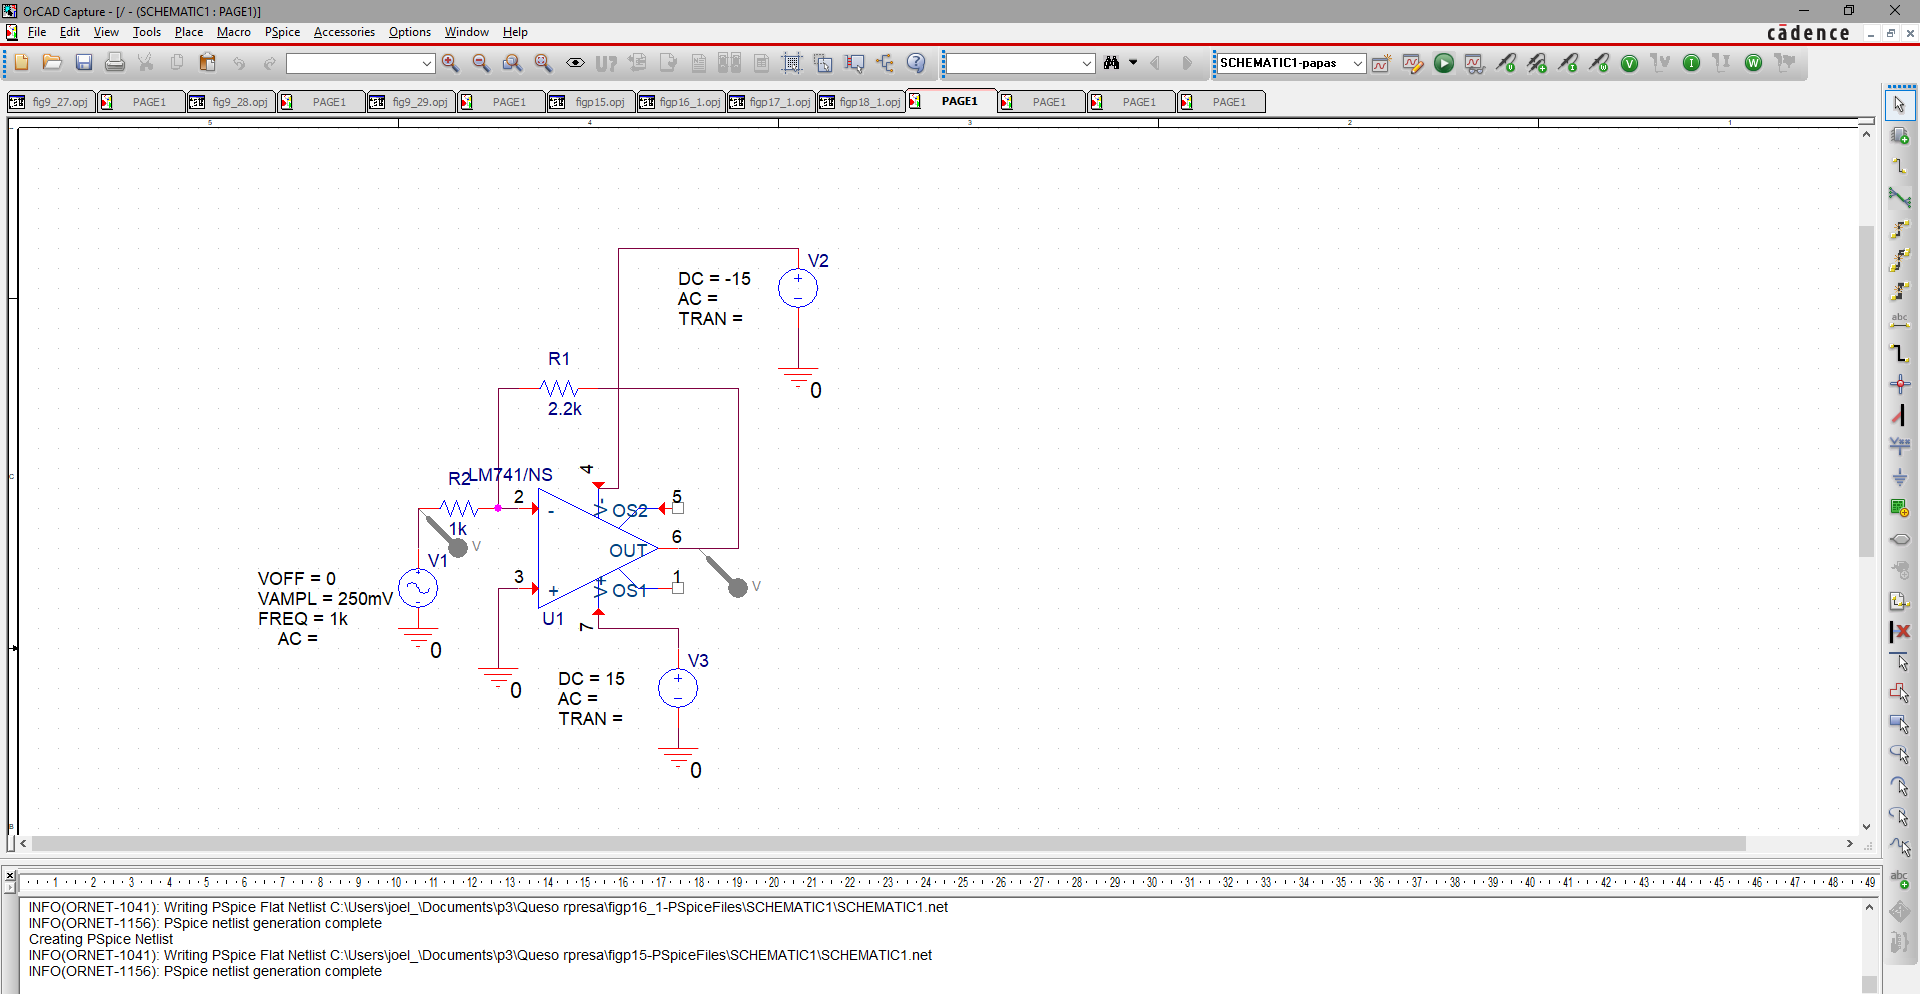
\includegraphics[width=18cm]{IMG/cir(5).png}
    \caption{Circuito 2 No inversor:}
    \label{fig:my_label}
\end{figure}
\begin{figure}[htbp]
    \centering
    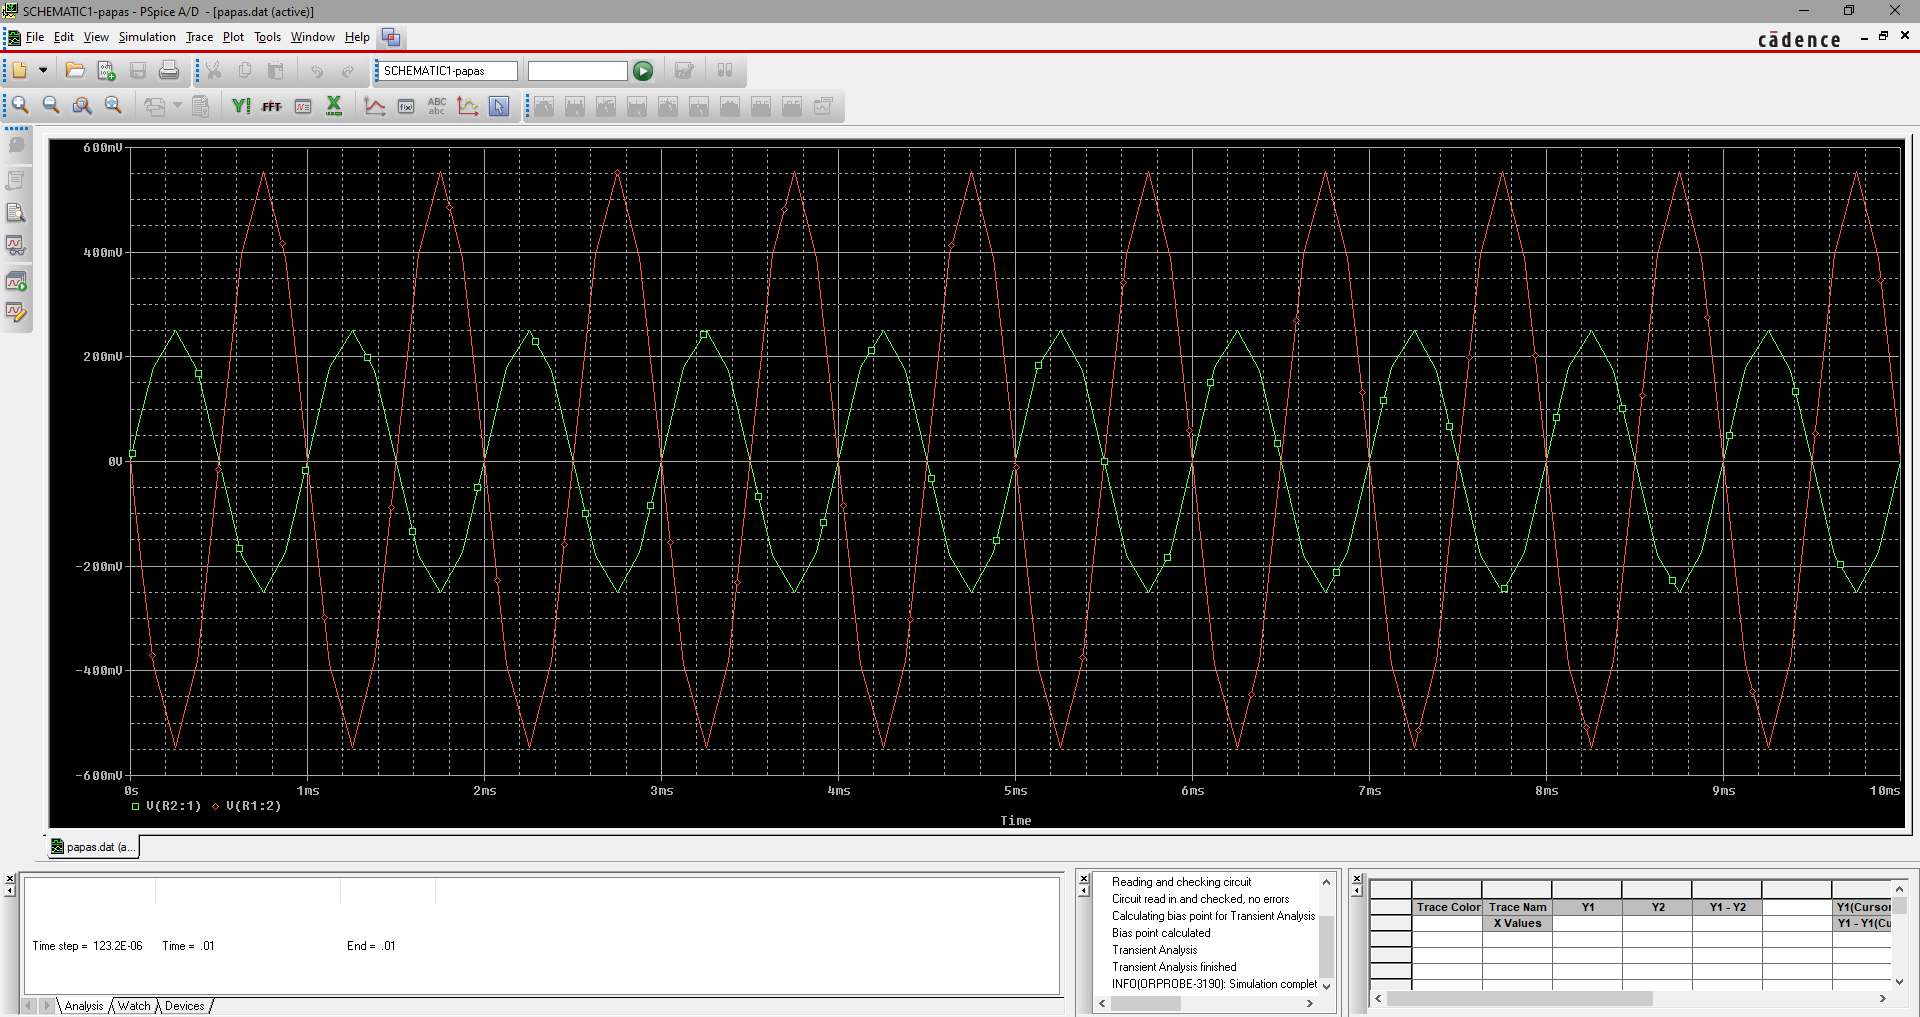
\includegraphics[width=18cm]{IMG/ond(1).png}
    \caption{Onda 2 No inversa: }
    \label{fig:my_label}
\end{figure}

%circuito 3 onda 3 cir 3 ond 3
\begin{figure}[htbp]
    \centering
    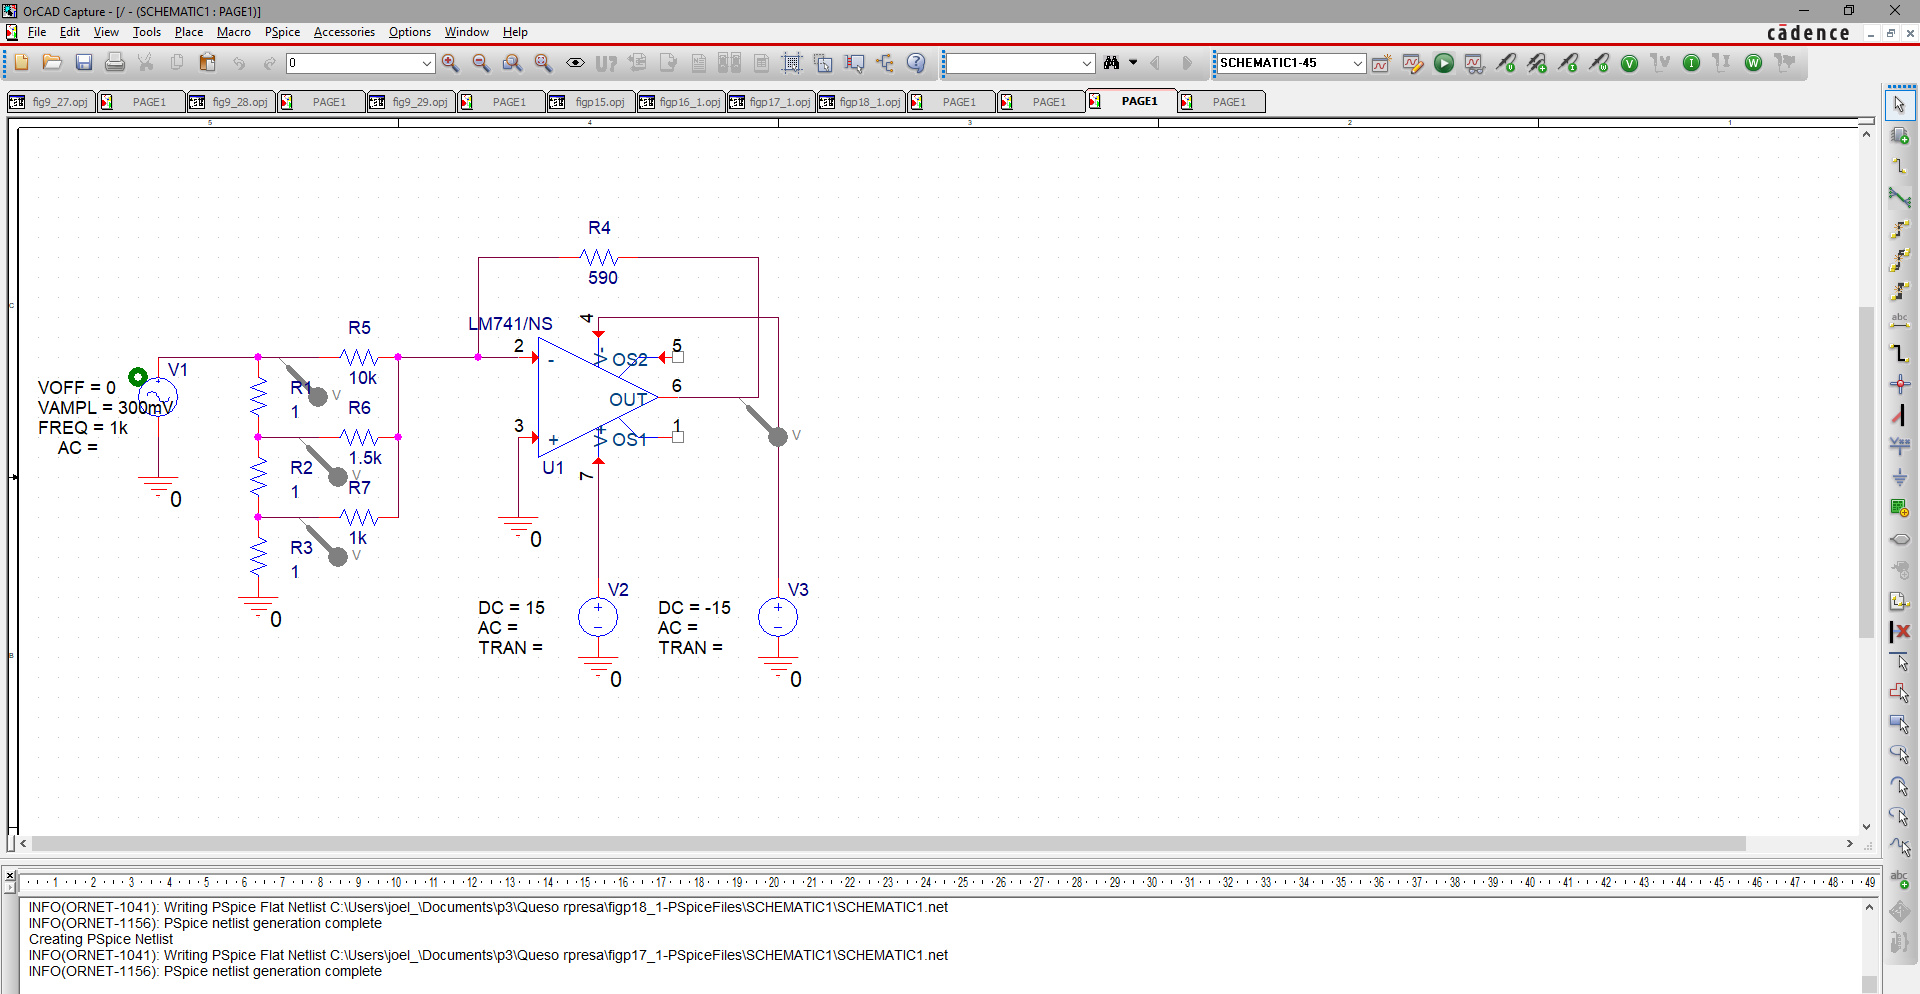
\includegraphics[width=18cm]{IMG/cir(3).png}
    \caption{Circuito 3: Sumador}
    \label{fig:my_label}
\end{figure}
\begin{figure}[htbp]
    \centering
    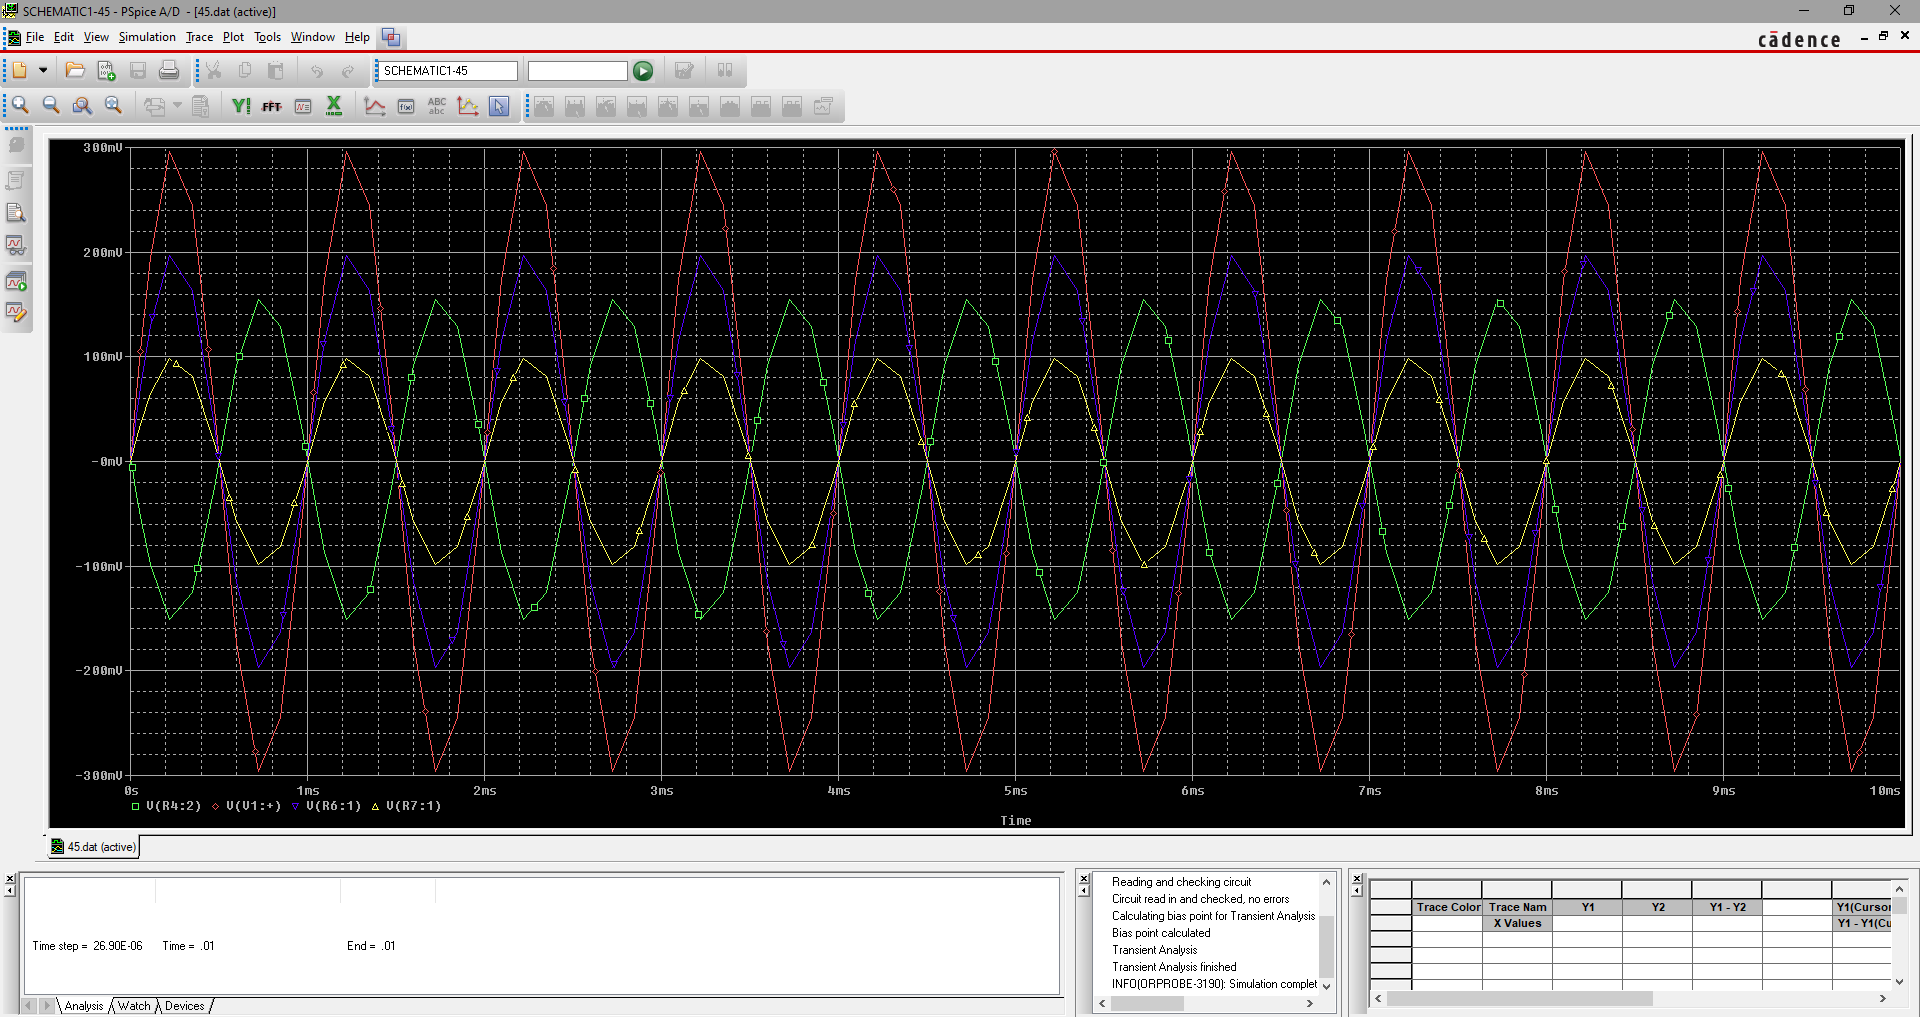
\includegraphics[width=18cm]{IMG/ond(3).png}
    \caption{Onda 3: Sumador}
    \label{fig:my_label}
\end{figure}

%circuito 4 onda 4 cir 2 ond 2
\begin{figure}[htbp]
    \centering
    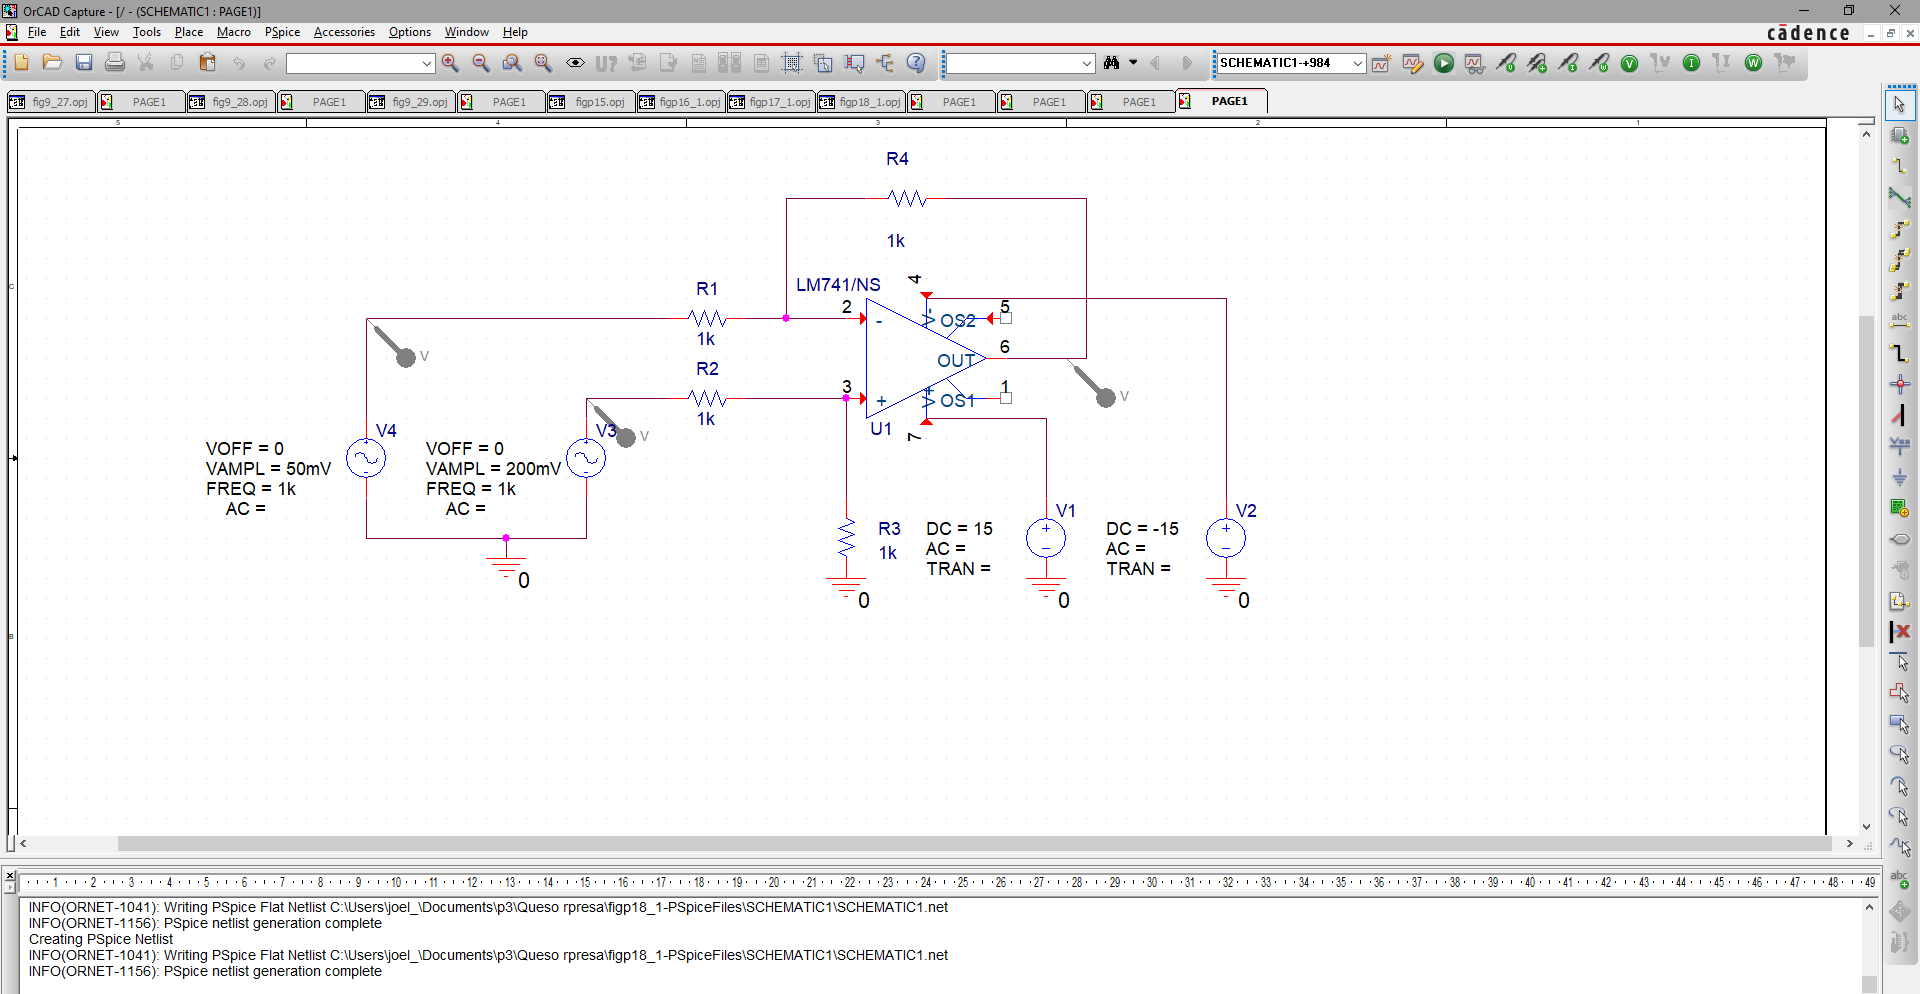
\includegraphics[width=18cm]{IMG/cir(2).png}
    \caption{Circuito 4 restador:}
    \label{fig:my_label}
\end{figure}
\begin{figure}[htbp]
    \centering
    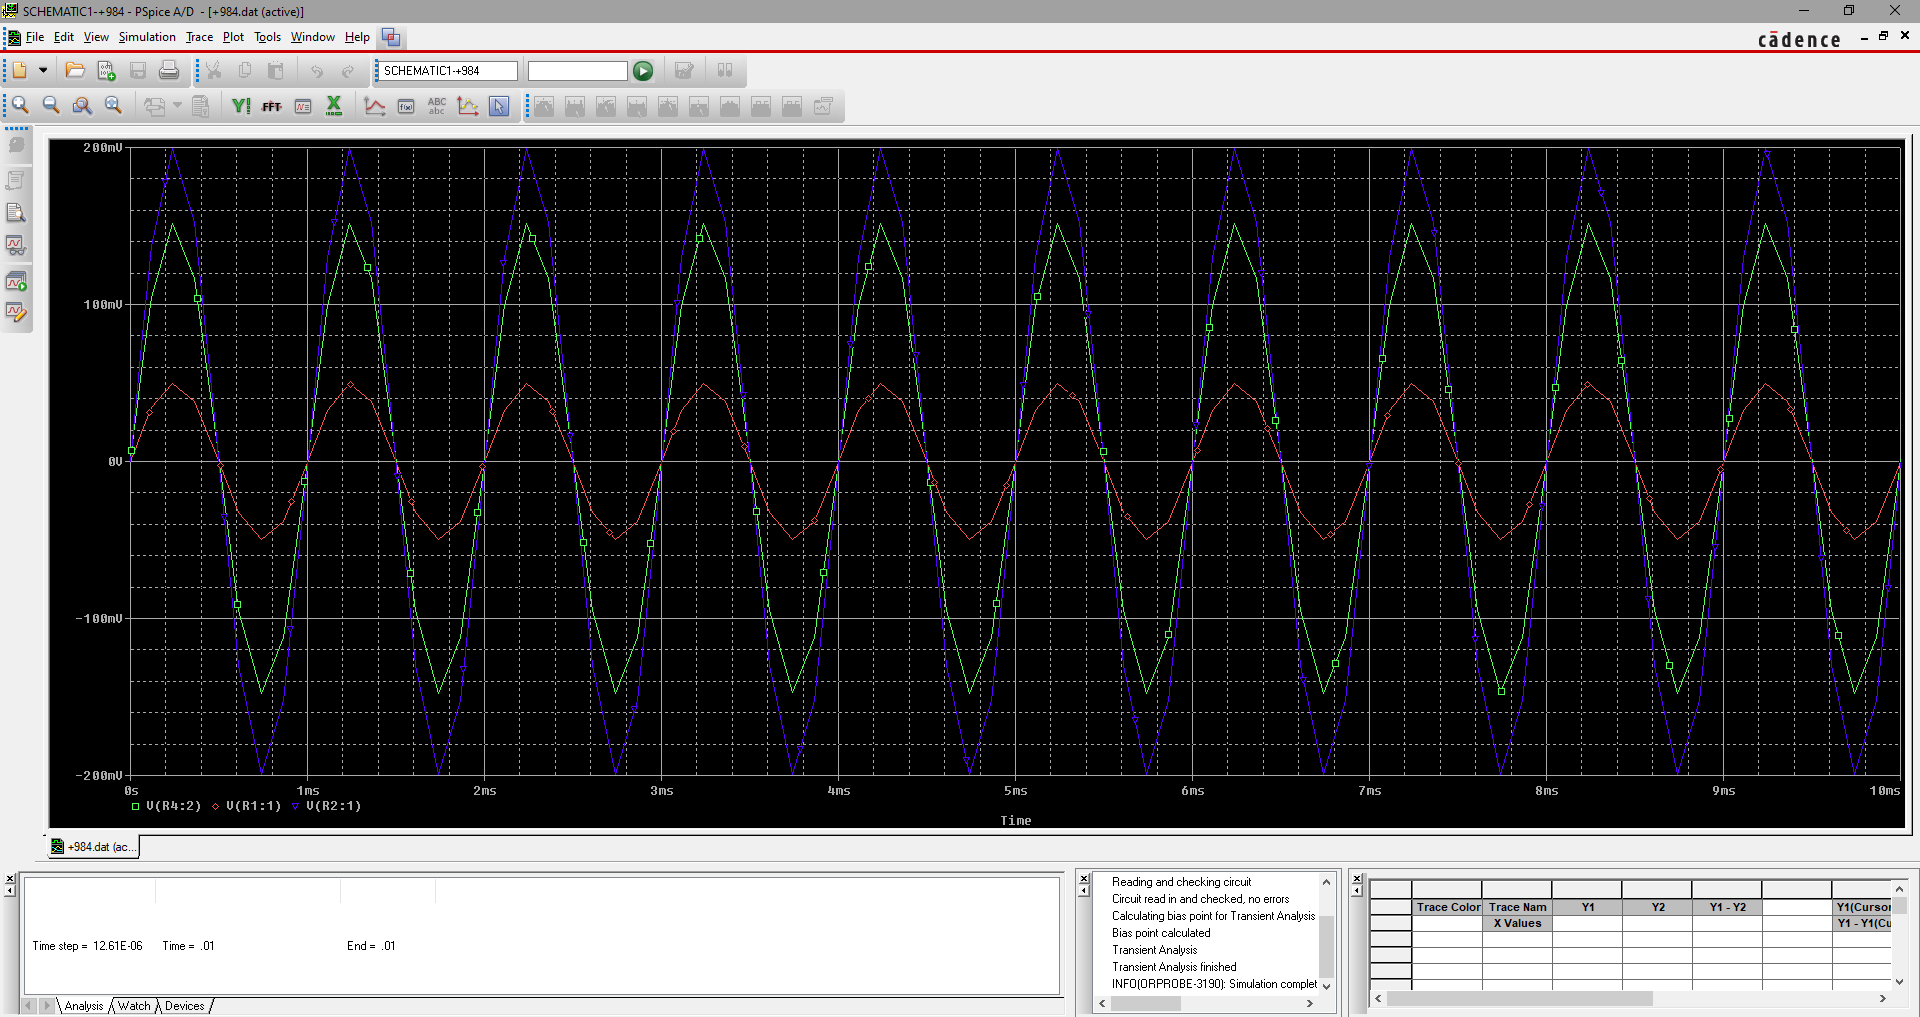
\includegraphics[width=18cm]{IMG/ond(2).png}
    \caption{Onda 4 restada: }
    \label{fig:my_label}
\end{figure}

%circuito 5 onda 5 cir 1 ond 4
\begin{figure}[htbp]
    \centering
    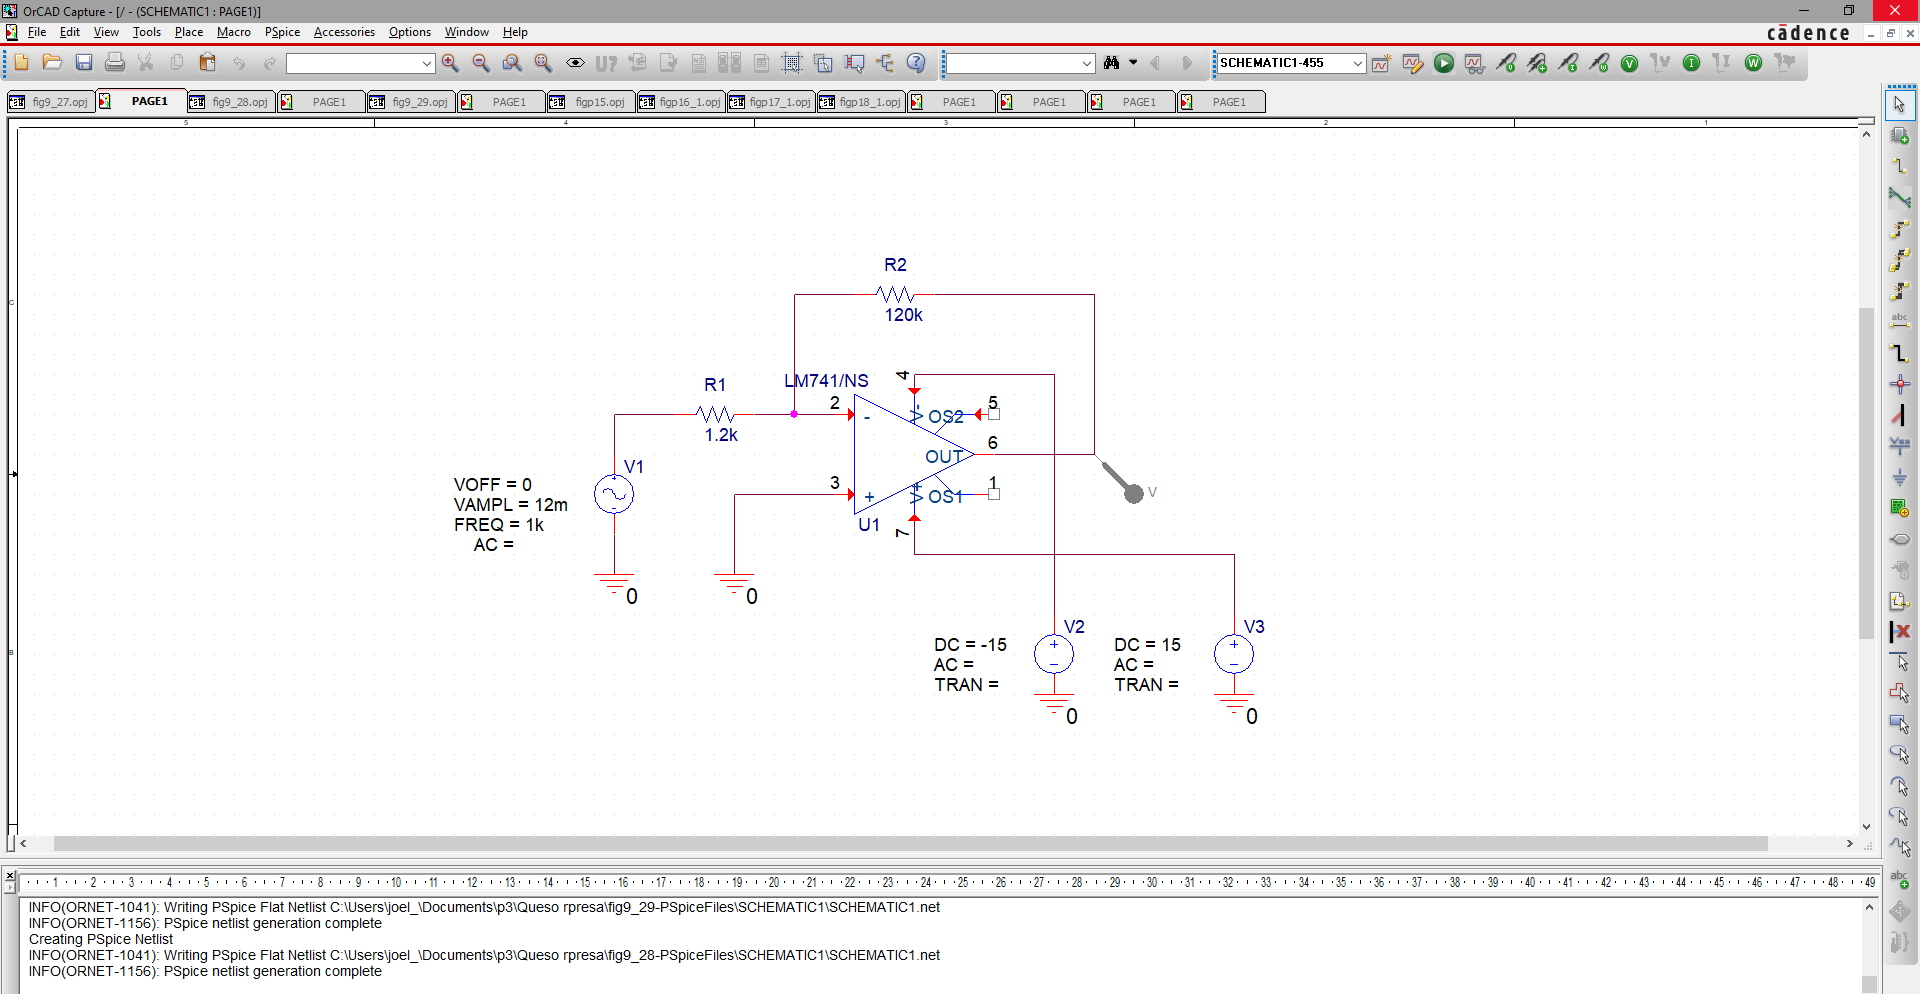
\includegraphics[width=18cm]{IMG/cir(1).png}
    \caption{Circuito 5 inversor:}
    \label{fig:my_label}
\end{figure}
\begin{figure}[htbp]
    \centering
    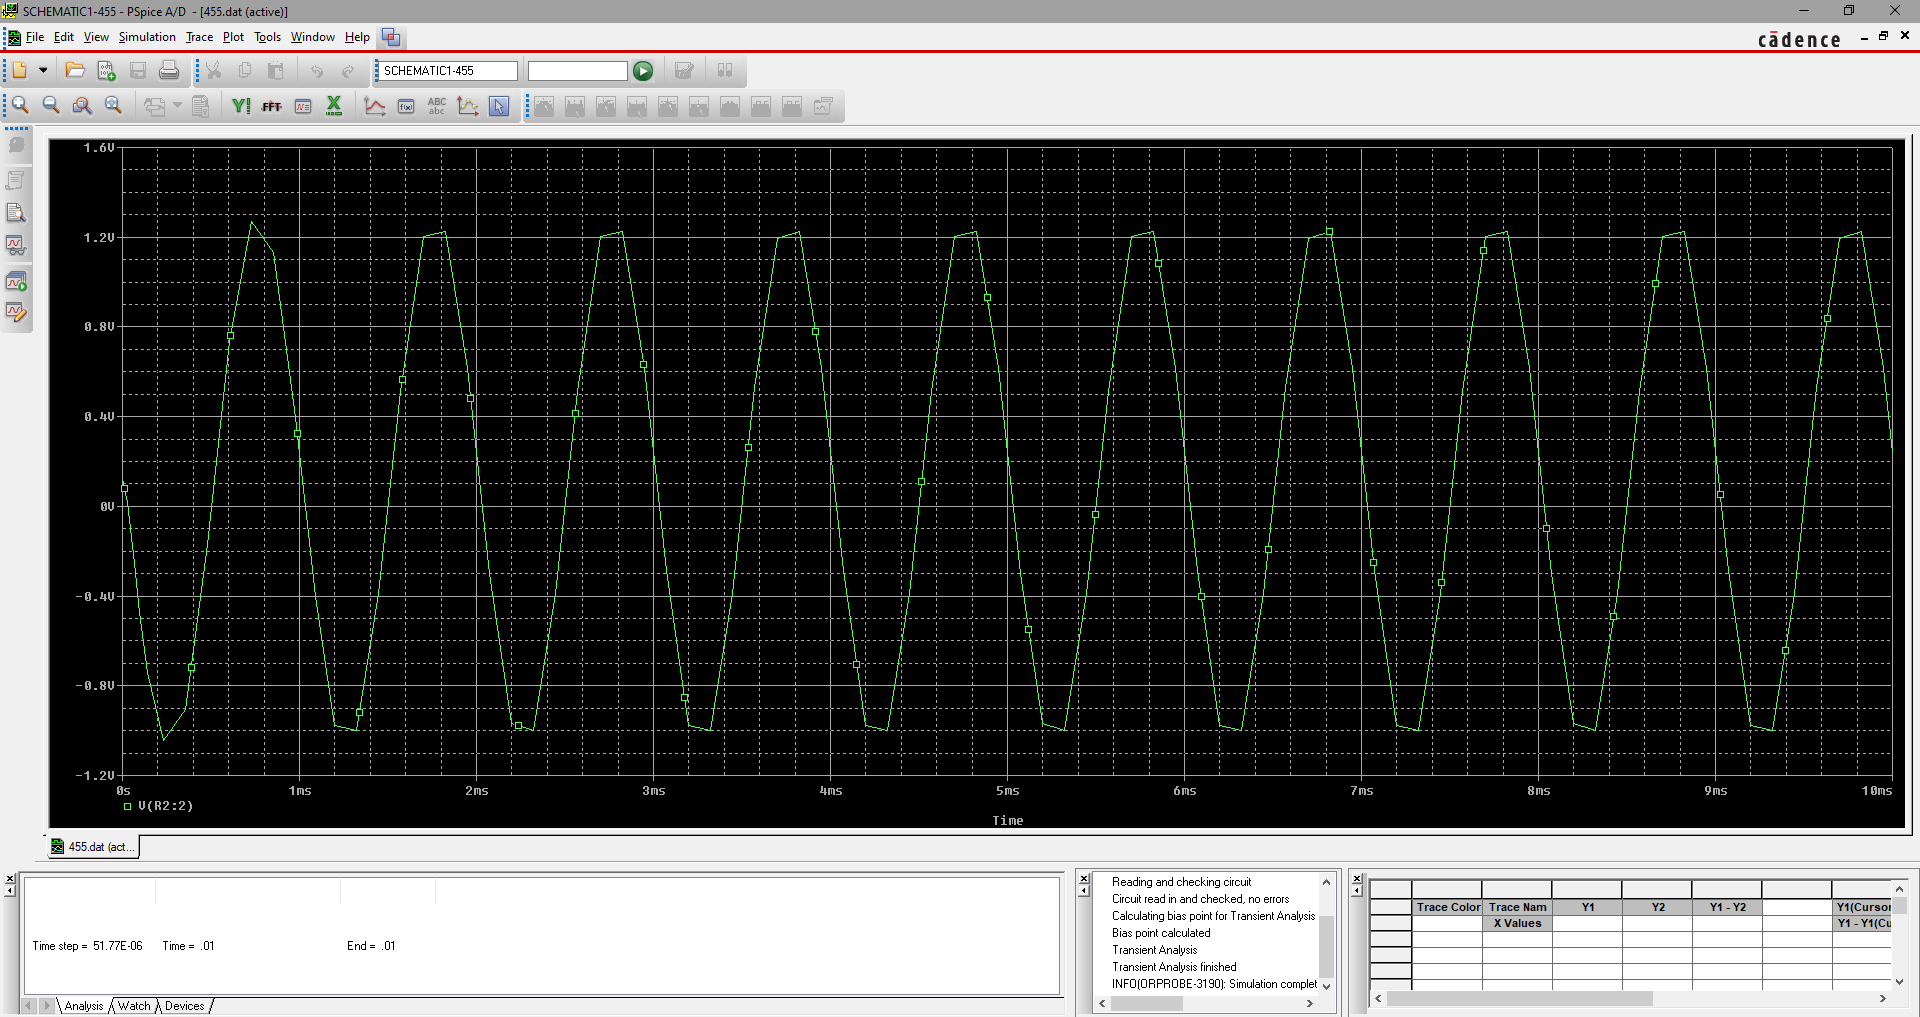
\includegraphics[width=18cm]{IMG/ond(4).png}
    \caption{Onda 5 inversa: }
    \label{fig:my_label}
\end{figure}

%circuito 6 onda 6 cir 7 ond 6
\begin{figure}[htbp]
    \centering
    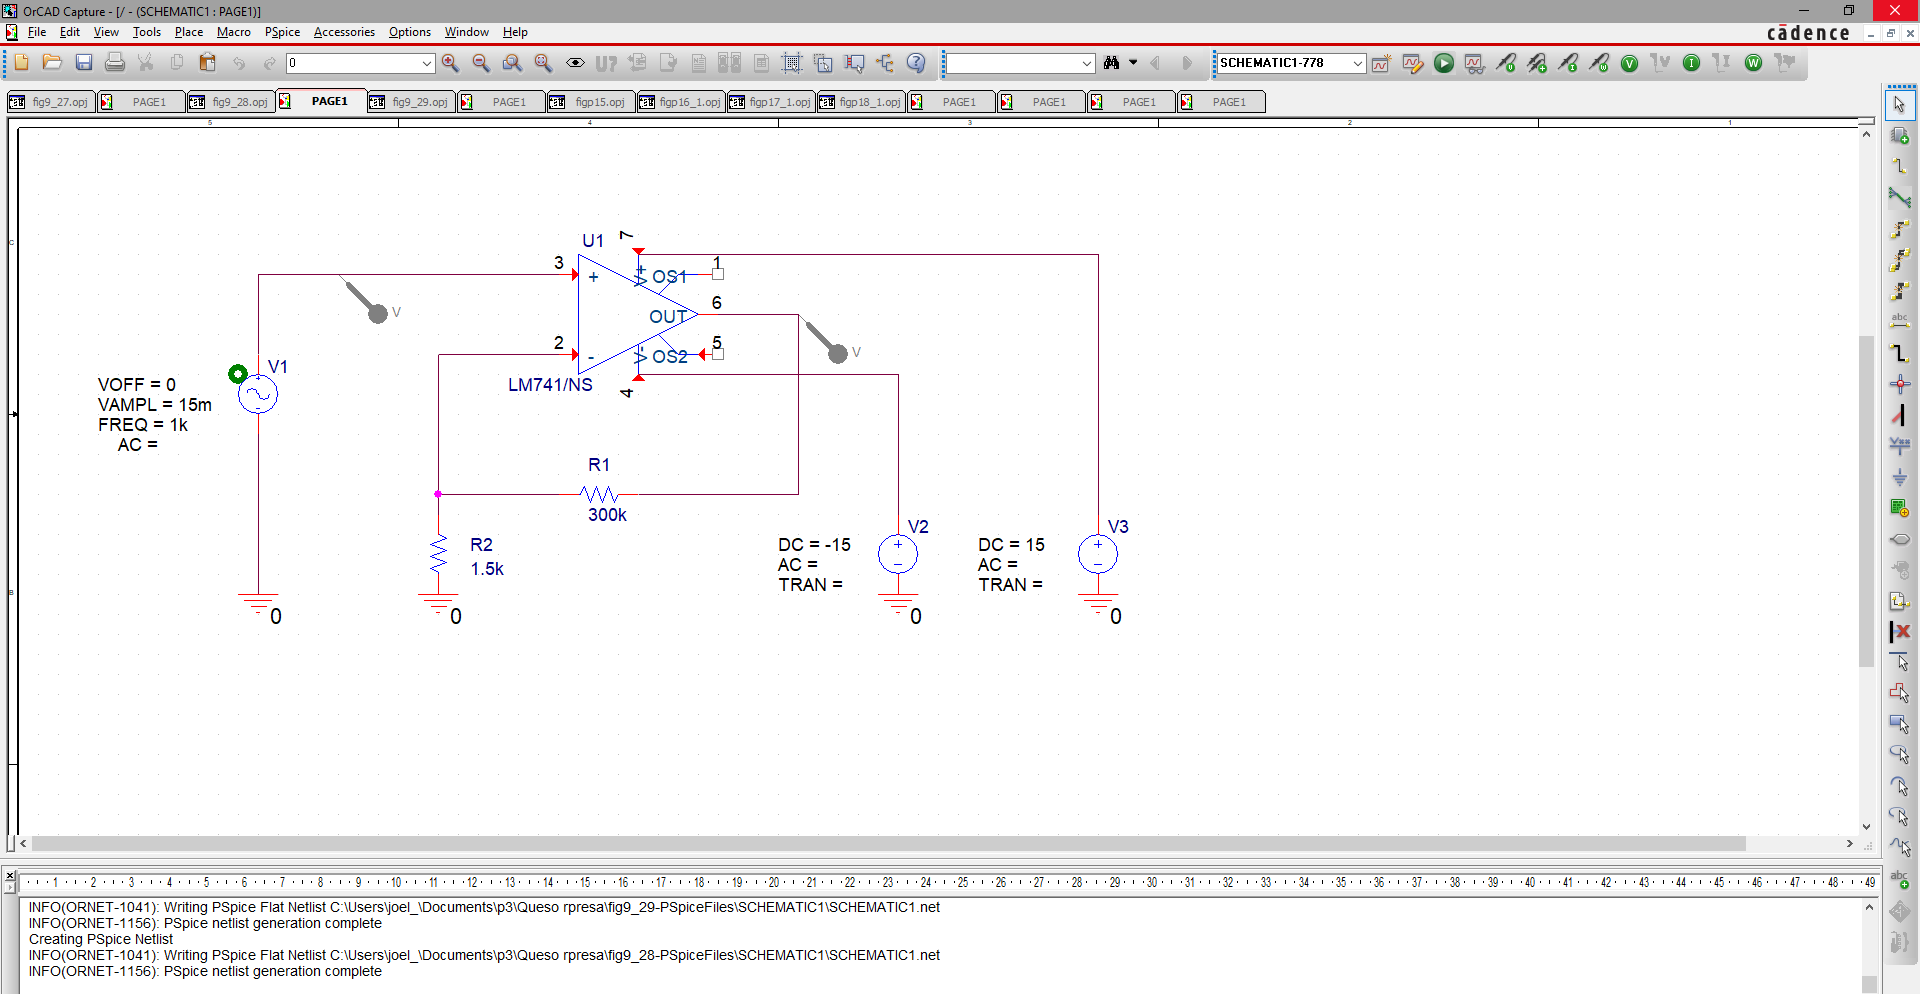
\includegraphics[width=18cm]{IMG/cir(7).png}
    \caption{Circuito 6 Inversor:}
    \label{fig:my_label}
\end{figure}
\begin{figure}[htbp]
    \centering
    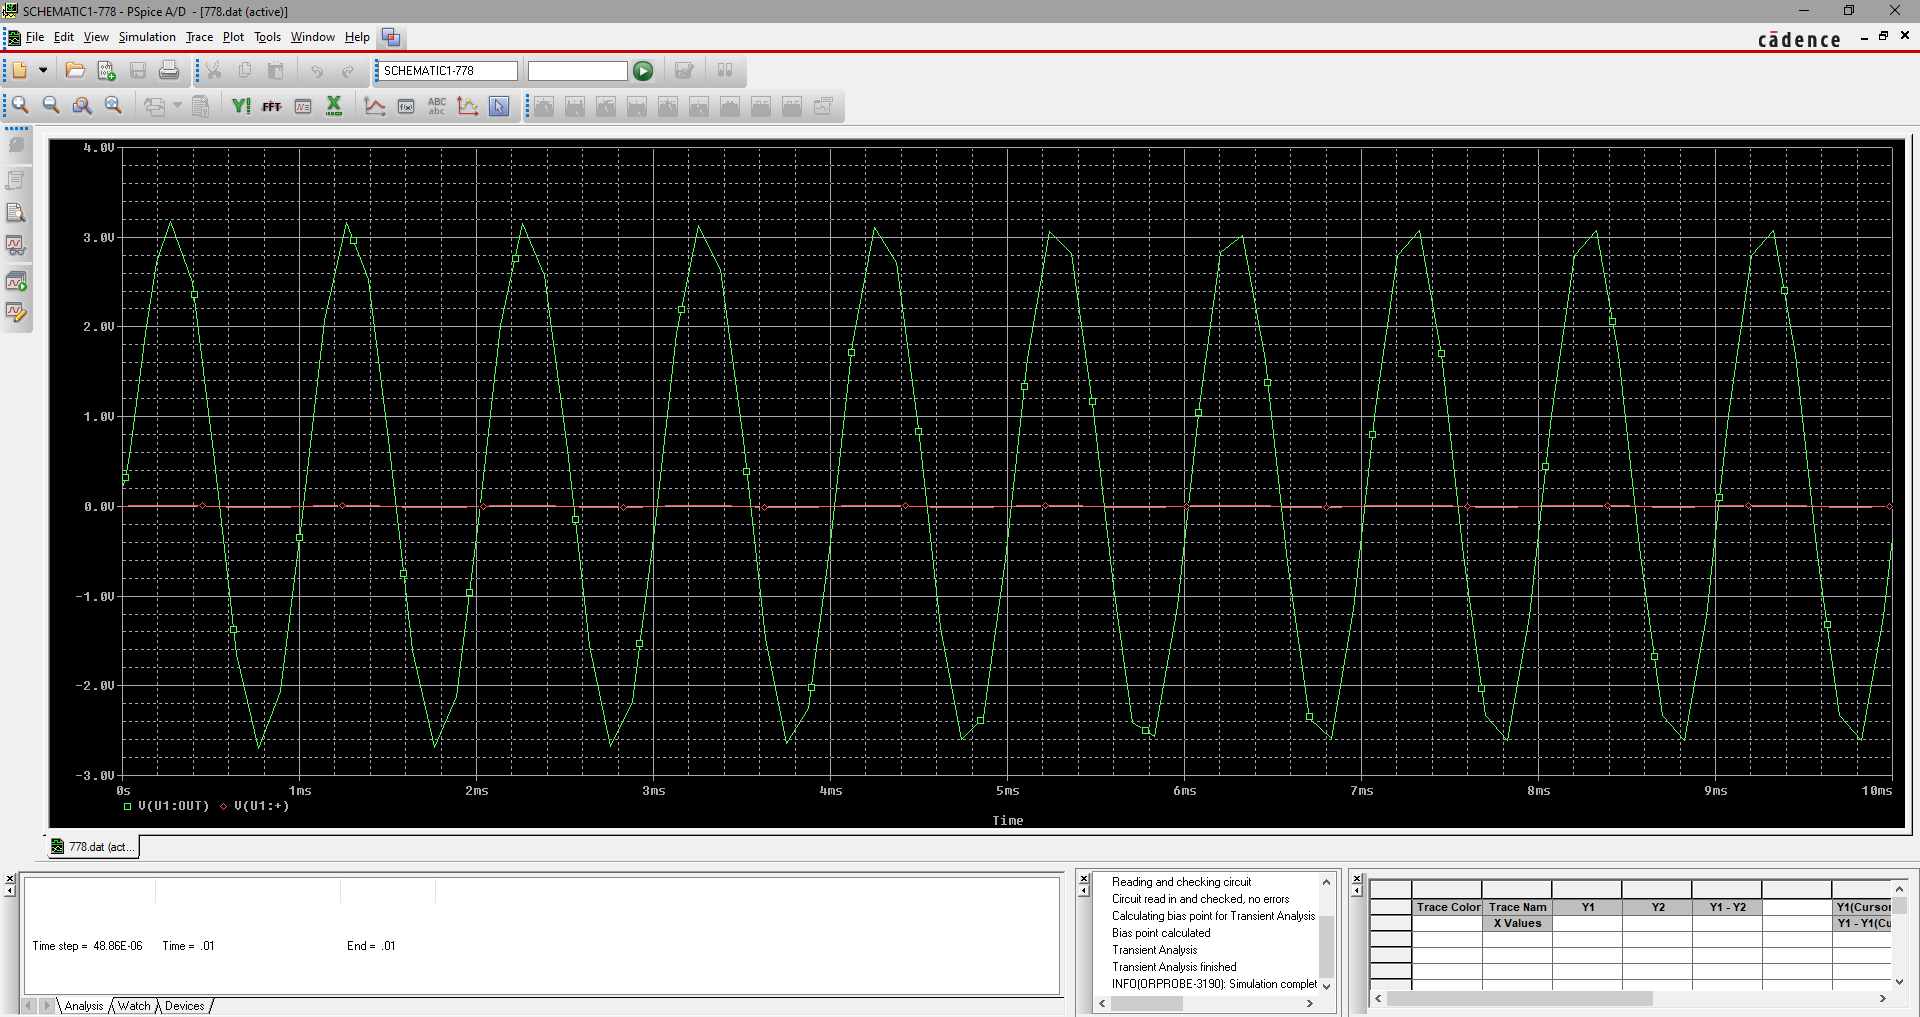
\includegraphics[width=18cm]{IMG/ond(6).png}
    \caption{Onda 6 Inversa: }
    \label{fig:my_label}
\end{figure}


%circuito 7 onda 7 cir 6 ond 5
\begin{figure}[htbp]
    \centering
    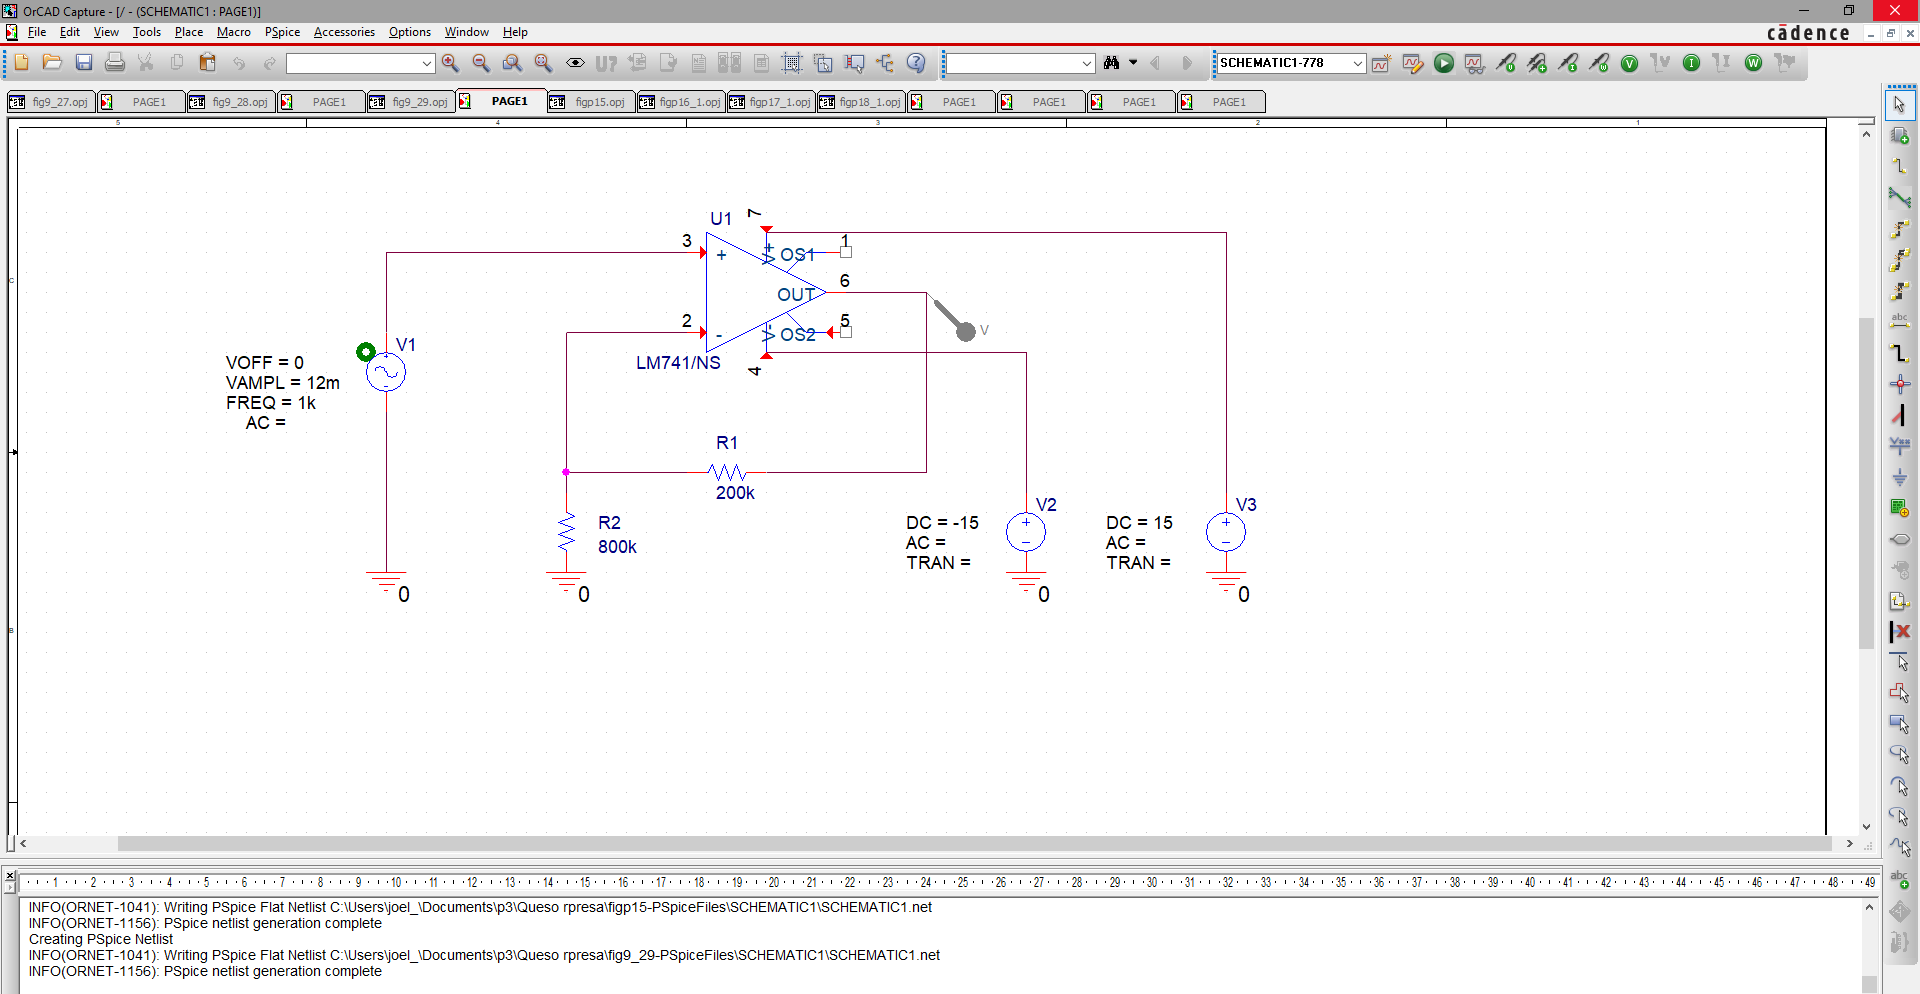
\includegraphics[width=18cm]{IMG/cir(6).png}
    \caption{Circuito 7 No inversor:}
    \label{fig:my_label}
\end{figure}
\begin{figure}[htbp]
    \centering
    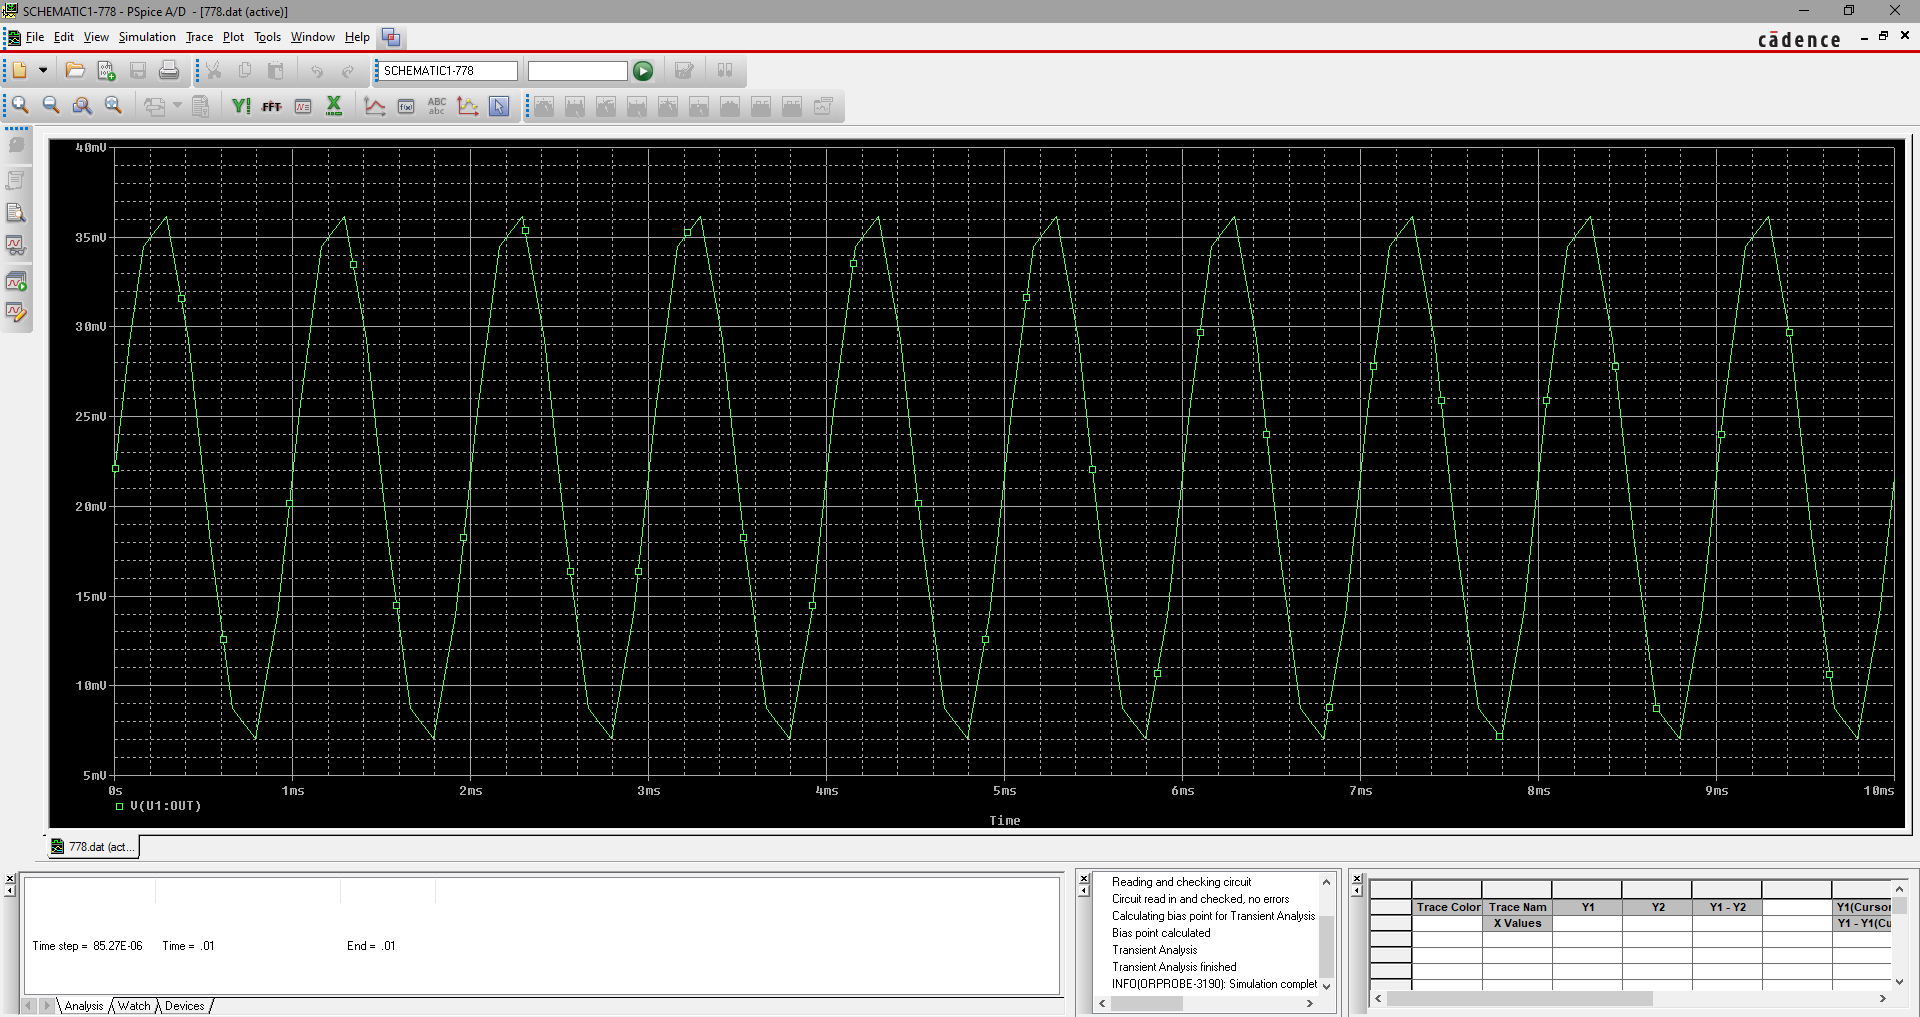
\includegraphics[width=18cm]{IMG/ond(5).png}
    \caption{Onda 7 No inversa: }
    \label{fig:my_label}
\end{figure}
\end{document}
